\section{Conceptos}

    \begin{enumerate}

        \item Da un ejemplo de Almacén de Datos (de acuerdo con tus intereses, no repetir lo visto en clase) y explica cómo se cumple la definición en tu ejemplo. Incluye:

            \begin{itemize}
                \item Orientación a temas
                \item Integración de datos
                \item Variabilidad en el tiempo
                \item No volatilidad
            \end{itemize}

            Diremos que existe una cadena minorista llamada ``\textit{Super Electronics}'' que, como su nombre dice, se dedica a comercialización de productos electrónicos de diversos tipos, como cables y adaptadores de corriente. Parecido a lo que haría una tienda como Radioshack o Steren.

Super Electronics tiene un Data Warehouse diseñado para el análisis de ventas y comportamiento del cliente. Este se explica de la siguiente manera:

\begin{itemize}

    \item \textbf{Orientación a temas}: En lugar de que el DW se organice en torno a operaciones de la empresa como ``pedidos'', ``facturación'' o ``gestión de inventario'', su DW está estructurado en torno a los temas principales del negocio, como Cliente, Producto, Ventas y Proveedor. Así, por ejemplo, se pueden analizar las ventas por tipo de artículo y/o por sucursal.

    \item \textbf{Integración de datos}: Los datos de su DW provienen de múltiples fuentes heterogéneas, es decir, de distintos sistemas tales como bases de datos relacionales, archivos planos, registros de transacciones antiguas. Estos datos se unifican para lograr tener una ``imagen corporativa única''. Esto implica limpiar y estandarizar con el fin de evitar las inconsistencias en convenciones de nomenclatura, unidades de medida y estructuras de codificación antes de almacenar los datos.

    \item \textbf{Variabilidad en el tiempo}: En lugar de reflejar valores actuales, como el saldo actual de una cuenta, su DW almacena información desde una perspectiva histórica (por ejemplo, los últimos 5 a 10 años, etc.). Esto lleva a que cada estructura de clave en el almacén contenga, implícita o explícitamente, un elemento de tiempo (como día, semana, mes o año).

    \item \textbf{No volatilidad}: El DW ésta pensado para solo ser consultado, no necesariamente modificado. Si ocurren cambios, se añade una nueva instantánea en lugar de sobrescribir el registro anterior, preservando así la historia de los mismos.

\end{itemize}


        \item Explica con tus propias palabras la diferencia entre un Almacén de Datos y:
            \begin{itemize}
    \item Una base de datos transaccional

        Un DW está diseñado para el análisis y la toma de decisiones estratégicas, organizando la información por ``temas'' (como clientes o productos, como mencionábamos en el ejercicio anterior), almacenando un historial a largo plazo. Por el contrario, una base de datos transaccional está diseñada para la operación diaria y eficiente de aplicaciones específicas, manejando datos actuales y volátiles que cambian constantemente.

    \item Un esquema estrella

        El DW es el repositorio corporativo completo que integra información de toda la organización, mientras que el esquema estrella es una técnica específica de modelado de datos utilizada dentro de los ``Data Marts'' para facilitar el análisis de la información contenida en el DW.

    \item Un cubo OLAP

        El DW almacena cantidades masivas de datos granulados con un horizonte de tiempo largo (i.e. 5 a 10 años), sirviendo como la fuente fundamental de datos. En cambio, un cubo OLAP organiza los datos del almacén de datos para que puedan analizarse más rápido, permitiendo explorarlos desde distintos puntos de vista, como por fecha, área o categoría, y facilitando las comparaciones.

    \item Un Data Lake

        El DW contiene datos estructurados, limpios e integrados que han pasado por un proceso de transformación para asegurar su calidad y consistencia. El Data Lake es más pensado como el \textit{intake} de datos crudos, donde se almacenan volúmenes de datos no necesariamente estructurarlos de manera previa y que no necesariamente cabrián en el DW.
  \end{itemize}

    \end{enumerate}


\section{Escenario}

    \begin{tcolorbox}[title=Contexto]
        El Instituto de Matemáticas de la Universidad Nacional Autónoma de México desarrolla
        y analiza modelos matemáticos mediante simulaciones numéricas, orientadas al estudio de
        ecuaciones diferenciales, sistemas dinámicos, procesos estocásticos y métodos numéricos.

        Cada ejecución de simulación genera información distribuida que se encuentra en registros del clúster, bitácoras de ejecución, archivos de resultados y reportes de uso de recursos computacionales. Actualmente, esta información no está integrada, lo que dificulta el análisis histórico y la toma de decisiones estratégicas.

        Por lo anterior, el Instituto te contrata para diseñar un Almacén de Datos que permita
        analizar el uso de recursos, el comportamiento de las simulaciones y su evolución a lo largo del tiempo.
    \end{tcolorbox}


    % \begin{enumerate}

    %     \item Menciona qué beneficios tendrá utilizar un Almacén de Datos en un entorno de cómputo científico. Justifica.

    %     \item Indica qué usuarios utilizarían este Almacén de Datos y con qué propósito. Justifica.

    %     \item Escribe al menos cinco preguntas que el Instituto desearía responder en términos de análisis.

    %     \item Describe qué datos históricos almacenaría el Data Warehouse del Instituto de Matemáticas y qué decisiones estratégicas apoyaría.

    %     \item Define el hecho principal del modelo multidimensional.

    %     \item Explica qué representa una fila en la tabla de hechos y da cinco ejemplos. Se consideran los siguientes niveles de granularidad para el hecho Ejecución de Simulación:

    %         \begin{itemize}
    %             \item Una fila por simulación científica
    %             \item Una fila por ejecución completa de simulación
    %             \item Una fila por paso iterativo interno
    %         \end{itemize}

    %     \item Selecciona la granularidad adecuada y justifica por qué es preferible a las demás.

    %     \item Explica cuándo sería adecuada una granularidad alta y cuándo una baja, incluyendo sus ventajas y desventajas.

    %     \item Dibuja el esquema estrella correspondiente al escenario. Considera que:

    %         \begin{itemize}
    %             \item Debe haber al menos cuatro medidas numéricas.
    %             \item Deben definirse al menos cinco dimensiones, incluidas Tiempo y Simulación.
    %             \item Deben indicarse los atributos relevantes de cada dimensión.
    %         \end{itemize}

    %     \item Describe las capas de la arquitectura de un Almacén de Datos.

    %     \item Explica el rol de cada capa en el contexto del cómputo científico.

    %     \item Indica dónde se implementa el modelo estrella.


    % \end{enumerate}
        \begin{enumerate}

        \item Menciona qué beneficios tendrá utilizar un Almacén de Datos en un entorno de cómputo científico. Justifica.

            \begin{itemize}
                \item \textbf{Integración de la información: } Reúne los datos dispersos entre las bitácoras, registros de clusters y archivos de resultados en un solo lugar.

                \item \textbf{Análisis dentro de un lapso de tiempo: } Permite el seguimiento de la evolución de los datos a lo largo de los años.

                \item \textbf{Repetibilidad: } Permite a los investigadores el comparar los resultados de simulaciones ejecutadas bajo las mismas condiciones.

                \item \textbf{Facilidad para hacer consultas: } Está optimizado para realizar análisis de forma eficiente por la estandarización de los datos.
            \end{itemize}

        \item Indica qué usuarios utilizarían este Almacén de Datos y con qué propósito. Justifica.

            \begin{itemize}
                \item \textbf{Investigadores y científicos: } Lo usarían para analizar el comportamiento de las simulaciones, identificar patrones y optimizar modelos matemáticos.

                \item \textbf{Directores del instituto: } Para la toma de decisiones basadas en la información que se obtiene en el DW.
            \end{itemize}

        \item Escribe al menos cinco preguntas que el Instituto desearía responder en términos de análisis.

            \begin{enumerate}
                \item ¿Cómo ha evolucionado la duración promedio de las simulaciones en los últimos dos años?

                \item ¿Cuál es la tasa de fallo de las simulaciones?

                \item ¿Qué condiciones de simulación son más probables para obtener un resultado exitoso?

                \item ¿Cuál es el porcentaje máximo histórico de recursos que se ha utilizado simultáneamente?

                \item Si dividiéramos todos las simulaciones realizadas en  periodos mensuales, ¿qué meses experimentaron un mayor crecimiento en la tasa de simulaciones exitosas?

            \end{enumerate}

        \item Describe qué datos históricos almacenaría el Data Warehouse del Instituto de Matemáticas y qué decisiones estratégicas apoyaría.

            \begin{itemize}
                \item \textbf{Datos históricos: } Tiempos de ejecución, uso de RAM por simulación, fechas de inicio y finalización, parámetros de las simulaciones y modelos.

                \item \textbf{Decisiones estratégicas: } Priorizar proyectos de investigación de alta demanda.
            \end{itemize}

        \item Define el hecho principal del modelo multidimensional.

            \textbf{Hecho principal: } Ejecución de simulaciones. \\
            Este hecho define el evento en donde un investigador toma un modelo (ecuaciones diferenciales, procesos estocásticos) para realizar una sola ejecución de simulación.

        \item Explica qué representa una fila en la tabla de hechos y da cinco ejemplos.\\
        Es el nivel de detalle que el sistema es capaz de analizar. En particular, cada fila contendrá datos de interés sobre una sola ejecución de la simulación realizada.

        \begin{figure}[h]
            \centering
            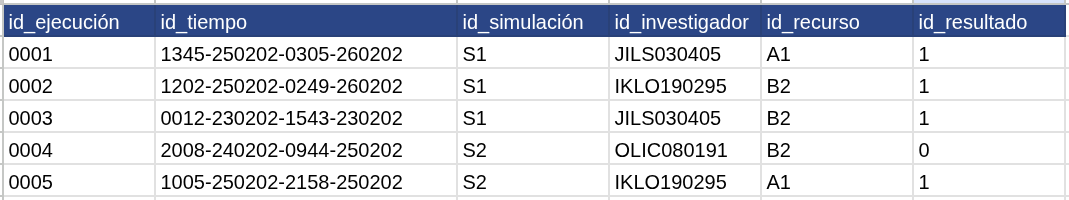
\includegraphics[width=0.8\textwidth]{imagenes/fact_table_rows_examples.png}
            \caption{Ejemplo de las filas de la tabla de hechos}
            \label{ejec}
        \end{figure}

        Por ejemplo, para la primera fila (ejecución):
        \begin{itemize}
            \item Se realiza la ejecución con id \texttt{0001}.
            \item La ejecución se realizó en el tiempo marcado con el id \texttt{1345-25202-0305-260202} (en este caso modelado como llave inteligente de la dimensión \texttt{Tiempo}), que representa que el inicio fue a las 13:45 del 25-02-02, y finalizó a las 03:05 del 26-02-02.
            \item La fila corresponde a una ejecución de la simulación con id \texttt{S1}.
            \item La ejecución la realizó el investigador con iniciales de CURP \texttt{JILS030405}.
            \item Esta ejecución fue procesada en el recurso con id \texttt{A1}.
            \item El resultado de esta ejecución fue 1 (éxito).
        \end{itemize}

        \item Se consideran los siguientes niveles de granularidad para el hecho Ejecución de Simulación:

            \begin{itemize}
                \item Una fila por simulación científica.
                \item Una fila por ejecución completa de simulación.
                \item Una fila por paso iterativo interno.
            \end{itemize}

        Selecciona la granularidad adecuada y justifica por qué es preferible a las demás.

        Para este escenario, una fila por ejecución completa de simulación es conveniente ya que permite analizar el rendimiento y si el resultado fue exitoso o no en cada ejecución. En cambio por simulación científica es muy general y perdemos el detalle de cada intento, mientras que por paso iterativo aporta un nivel de granularidad excesivo que saturaría el almacenamiento sin aportar información útil para la toma de decisiones.

        \item Explica cuándo sería adecuada una granularidad alta y cuándo una baja, incluyendo sus ventajas y desventajas.\\
        Una granularidad alta es adecuada cuando necesitamos almacenar los datos de manera más precisa. Este tipo de granularidad es adecuada, cuando al usuario necesita analizar profundamente cada hecho, por ejemplo para realizar Deep Learning. Las ventajas que ofrece la granularidad alta son una capacidad de análisis grande, sin embargo será necesario sacrificar costos de almacenamiento y velocidad. \\
        Por otro lado, la granularidad baja es deseable cuando se requieren resúmenes o dashboards de alto nivel, es decir, que se desea dar resultados más generales que resuman las preguntas de negocio. La ventaja que ofrece sería su gran velocidad de consulta y el poco costo de implementación. Aunque esto, trae consigo desventajas como muy poca flexibilidad en cuanto a la capacidad de consulta y análisis.



        \item Dibuja el esquema estrella correspondiente al escenario. Considera que:

            \begin{itemize}
                \item Debe haber al menos cuatro medidas numéricas.
                \item Deben definirse al menos cinco dimensiones, incluidas Tiempo y Simulación.
                \item Deben indicarse los atributos relevantes de cada dimensión.
            \end{itemize}

            \begin{figure}[H]
                \centering
                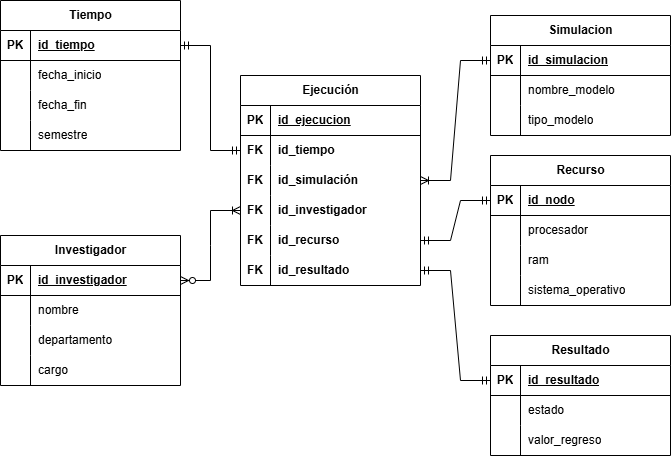
\includegraphics[width=0.8\textwidth]{imagenes/ejecucion.drawio.png}
                \caption{Esquema estrella de una ejecución de una simulación}
                \label{ejec}
            \end{figure}

        \item Describe las capas de la arquitectura de un Almacén de Datos.

        Básicamente, la arquitectura se divide en 4 capas principales que marcan el camino de los datos desde que salen de los sistemas originales hasta que se usan para reportes

        \begin{itemize}
            \item \textbf{Data Source}: Aquí es de donde viene todo. Son los sistemas transaccionales (OLTP), archivos o bases de datos externas que tienen la información sin procesar.

            \item \textbf{Data Staging}: Es como una zona de paso. Aquí se hace el proceso de ETL (Extraer, Transformar y Cargar), donde se limpian, estandarizan y acomodan los datos para que no tengan errores antes de guardarlos.

            \item \textbf{Data Storage}: Es el núcleo del sistema. Aquí ya vive el Data Warehouse centralizado y los Data Marts, los cuales son fragmentos de esa información ya organizada y lista para ser consultada de forma histórica.

            \item \textbf{Data Presentation}: Es la capa que ve el usuario final. Se usa para hacer el análisis de datos, sacar reportes  o aplicar minería de datos para encontrar patrones útiles para el negocio.
        \end{itemize}

        \item Explica el rol de cada capa en el contexto del cómputo científico.

        \begin{itemize}
            \item \textbf{Data Source}: En el contexto científico, esta capa agrupa todos los sistemas que generan datos durante las investigaciones, es decir, donde se producen los datos sin procesar como en los registros del clúster, bitácoras de ejecución de los modelos matemáticos y archivos de resultados de las simulaciones.

            \item \textbf{Data Staging}: En este caso, debido a las múltiples fuentes de datos, esta capa se encarga de estandarizar los datos mediante parsers, cálculos y transformaciones. Luego se realiza la carga de estos datos a la siguiente capa.

            \item \textbf{Data Storage}: Aquí se guarda una copia todos los datos históricos obtenidos, el cuál se actualiza periódicamente o conforme la Institución lo vaya requiriendo.

            \item \textbf{Data Presentation}: Se presenta ante los investigadores herramientas que permiten realizar un análisis del negocio, tales como gráficas, reportes, etc.
        \end{itemize}

        \item Indica dónde se implementa el modelo estrella. \\
        Este esquema (hecho y dimensiones) se encuentra únicamente en la capa de Storage, esto debido a que las capas anteriores (Source y Staging) viven y se trabajan con datos crudos y temporales. Tampoco se encuentran en la capa Presentation, ya que esta únicamente sirve de lectura. \\
        Es así como en la capa de Storage vive el modelo estrella, ya que como vimos, esta es la toma los datos (ya estandarizados) y los guarda de forma desnormalizada para que puede realizar las consultas necesarias para el análisis que se presentara en la capa de presentación.

    \end{enumerate}

\section{Detección de errores}

Plantea y describe dos errores de diseño posibles en un Almacén de Datos para el escenario anterior. Los errores no deben impedir la ejecución de consultas, pero sí producir resultados incorrectos o engañosos. Para cada error, indica:

    \begin{itemize}
        \item Un ejemplo de consulta donde el problema sea evidente.
        \item Cómo corregirías el error (ETL o modelo). Escribe detalladamente los pasos a seguir,
        así como tu solución.
    \end{itemize}


    \begin{enumerate}
        \item \textbf{Atribución incorrecta de recursos por actualización en la dimensión}: En la dimensión Recurso se actualizan las características del hardware, en particular la RAM, sobrescribiendo el valor anterior sin guardar historial.   De esta manera al realizar la consulta ¿Cuál era el rendimiento de las simulaciones cuando los nodos tenían solo 32GB de RAM?, si todos los nodos se actualizaron a 64GB y se sobrescribió el dato, el reporte histórico asociará ejecuciones históricas con una configuración de hardware que no existía en el momento en que ocurrieron, lo cual genera una inconsistencia en los datos históricos y genera una representación distorsionada de las condiciones reales bajo las cuales se ejecutaron las simulaciones, afectando el análisis de eficiencia.

        La solución a esto consiste en cambiar la dimensión Recurso a una Dimensión de variación lenta de tipo 2. Para esto agregamos las columnas fecha\_inicio, fecha\_fin y estatus, así cuando un nodo se actualice como en este caso particular la RAM, no se debe sobrescribir, en su lugar se debe cerrar el registro actual con la fecha de hoy y crear una nueva fila con la nueva configuración.

        \item \textbf{Ambigüedad en la categorización de estados de salida por mapeo genérico}: En la dimensión Resultado, el proceso de ETL mapea cualquier código de salida distinto de cero como un Fallo genérico en el atributo \textit{estado}. De esta manera, al realizar la consulta ¿Cuál es la eficiencia de los modelos de Ecuaciones Diferenciales?, si el reporte muestra una alta tasa de fallos pero no distingue entre un error matemático y una interrupción por mantenimiento del clúster, el reporte histórico mostrará una baja eficiencia del modelo, lo cual genera una interpretación engañosa de la calidad del algoritmo y podría llevar a la decisión estratégica incorrecta de abandonar una investigación útil basándose en fallos de infraestructura y no de lógica.

        La solución a esto consiste en ajustar la lógica de transformación en la capa de Staging para realizar un análisis de los logs de ejecución antes de la carga. Para esto, se debe reclasificar el atributo \textit{estado} en categorías específicas por ejemplo, fallo matemático, interrupción de hardware, cancelación Manual, etc. Así, el proceso ETL asignará la llave foránea correcta en la tabla de hechos, permitiendo que el Almacén de Datos refleje con precisión la causa raíz de cada evento.
    \end{enumerate}

